\documentclass[11pt]{article}
\usepackage[margin=0.85in]{geometry}
\usepackage{amsmath,amssymb,booktabs,graphicx,tikz}
\usepackage[hidelinks]{hyperref}
\usetikzlibrary{arrows.meta}
\setlength{\parindent}{0pt}
\setlength{\parskip}{7pt}
\newcommand{\parttitle}[1]{\par\textbf{#1}\par}
\newcommand{\dataplot}[1]{%
\begin{tikzpicture}[x=0.43cm,y=0.43cm]
\draw[step=1,gray!20,very thin] (0,0) grid (10,8);
\draw[-{Latex}] (0,0)--(10.5,0) node[right] {$x_1$};
\draw[-{Latex}] (0,0)--(0,8.5) node[above] {$x_2$};
\foreach \x/\y in {1/6,2/7,3/6.8,3/5.8,2/5,1.5/0.5}
  \fill[red!75!black] (\x,\y) circle (2.5pt);
\foreach \x/\y in {2/6,6/6.5,6.2/2,6.8/1.8,6/1,7/1,8/2.4,8.2/1.2}{
  \draw[green!45!black,line width=1.5pt] (\x-0.13,\y-0.13)--(\x+0.13,\y+0.13);
  \draw[green!45!black,line width=1.5pt] (\x-0.13,\y+0.13)--(\x+0.13,\y-0.13);
}
#1
\end{tikzpicture}}
\begin{document}
\begin{center}
{\LARGE CIS 5190: Homework 2}\\[5pt]
{\large Written Answers}
\end{center}

\section*{Use of AI Tools}
I used OpenAI Codex. It wrote a first draft of the answers, did the calculations, and made the LaTeX figures. This can save time, but it can also let me skip steps. I need to check each answer and explain each step myself to learn the material.

\section*{Time Spent}
These are rough estimates, not measured times.
\begin{center}
\begin{tabular}{lr}
\toprule
Part & Estimated time (hours)\\
\midrule
Reading the assignment & 0.25\\
Question 1 & 0.75\\
Question 2 & 0.50\\
Question 3 & 0.50\\
Question 4 & 0.50\\
Question 5 & 0.75\\
Question 6 & 0.75\\
\midrule
Total & 4.00\\
\bottomrule
\end{tabular}
\end{center}

\newpage
\section*{Question 1: Logistic Regression}
The boundary is $\beta_0+\beta_1x_1+\beta_2x_2=0$. Red dots have $y=1$ and green crosses have $y=0$. The plots below copy the point positions approximately. The lines show approximate fitted boundaries; the axes use an arbitrary scale.

\begin{center}
\begin{minipage}[t]{0.48\textwidth}
\centering
\textbf{(a) No strong penalty}\\[4pt]
\dataplot{\draw[blue,thick] (3.25,0)--(3.70,8);}

Predict 1 to the left of the line.\\
\textbf{1 wrong point:} the green cross inside the red group.
\end{minipage}\hfill
\begin{minipage}[t]{0.48\textwidth}
\centering
\textbf{(b) Strong penalty on $\beta_0$}\\[4pt]
\dataplot{\draw[blue,thick] (0,0)--(5.41,8);}

Here $\beta_0=0$, so the line must pass through the origin. Predict 1 above the line.\\
\textbf{2 wrong points:} the green cross inside the red group and the low red dot.
\end{minipage}

\vspace{18pt}
\begin{minipage}[t]{0.48\textwidth}
\centering
\textbf{(c) Strong penalty on $\beta_1$}\\[4pt]
\dataplot{\draw[blue,thick] (0,4.62)--(10,4.62);}

Here $\beta_1=0$, so the boundary is horizontal. Predict 1 above the line.\\
\textbf{3 wrong points:} the two high green crosses and the low red dot.
\end{minipage}\hfill
\begin{minipage}[t]{0.48\textwidth}
\centering
\textbf{(d) Strong penalty on $\beta_2$}\\[4pt]
\dataplot{\draw[blue,thick] (3.53,0)--(3.53,8);}

Here $\beta_2=0$, so the boundary is vertical. Predict 1 to the left of the line.\\
\textbf{1 wrong point:} the green cross inside the red group.
\end{minipage}
\end{center}

\newpage
\section*{Question 2: Neural Networks}
\parttitle{(a) Zero initialization}
All units in the same hidden layer start the same and get the same updates. They cannot learn different features. This is the symmetry problem. With ReLU, zero inputs can also give zero gradients, so hidden units may not learn at all.

\parttitle{(b) Nonlinear activation}
Without a nonlinear activation, a stack of linear layers is still one linear map:
\[
W_2(W_1x+b_1)+b_2=(W_2W_1)x+(W_2b_1+b_2).
\]
A nonlinear activation lets the network learn nonlinear patterns and boundaries.

\parttitle{(c) Number of parameters}
The image has $40\times30=1200$ input values. Each unit has one bias.
\begin{align*}
\text{Hidden layer 1: }&1200\times64+64=76{,}864,\\
\text{Hidden layer 2: }&64\times32+32=2{,}080,\\
\text{Output layer: }&32\times10+10=330.
\end{align*}
The total is
\[
\boxed{76{,}864+2{,}080+330=79{,}274}.
\]

\newpage
\section*{Question 3: k Nearest Neighbors}
\parttitle{(a)(i) Two training points}
The boundary is the perpendicular bisector of the line segment joining the two points. Every point on this boundary is equally far from the two training points. Each side gets the label of its closer training point.

\parttitle{(a)(ii) Approximating a boundary}
Yes, for a usual boundary in a bounded region. Place many training points on both sides of the desired boundary, with the correct label on each side. Put points close to the boundary and close to each other. A finer set of points gives smaller nearest-neighbor regions, so the boundary can follow finer details.

\parttitle{(b) Setting $k=n$}
For regression, every query gets the mean of all training targets:
\[
\hat y(x)=\frac{1}{n}\sum_{i=1}^{n}y_i.
\]
For classification, every query gets the most common training label. A fixed rule handles ties. Neither answer depends on the query location.

\parttitle{(c) Bias and variance}
A small $k$ gives a flexible boundary. It usually has low bias and high variance because a few training points can change the answer.

A larger $k$ averages over more points. It usually raises bias and lowers variance. At $k=n$, the answer is constant, so local patterns are lost.

\newpage
\section*{Question 4: k Nearest Neighbors for Houses}
\parttitle{(a) Different feature scales}
Square footage may be in the thousands, while distance to a school may be only a few miles. Raw Euclidean distance is then mostly based on square footage.

Scale each feature, for example with
\[
z_j=\frac{x_j-\mu_j}{s_j}.
\]
Fit $\mu_j$ and $s_j$ on the training data, and use the same values for new data. Feature weights can also help if one feature matters more.

\parttitle{(b) Roof type}
Integer IDs create a false order and false distances. For example, IDs 0 and 2 are not necessarily less similar than IDs 0 and 1.

Use one-hot encoding. Each roof type gets its own binary column. Different roof types then have the same distance in the roof feature group. Scale or weight this group as needed.

\parttitle{(c) Curse of dimensionality}
In many dimensions, data become sparse. A small local region needs many more samples, and nearest neighbors may no longer be very close. Irrelevant features can also hide useful distances.

Digit images can still work well because their pixels are related. Real digit images occupy a much smaller set than all possible pixel arrays. Their useful dimension can be much lower than the number of pixels.

\newpage
\section*{Question 5: Decision Trees}
\parttitle{(a) Why use early stopping?}
Growing a large tree takes time and memory. Early stopping avoids many weak splits before they are made. Post-pruning can then remove more branches. A validation set is finite, so pruning may not remove every branch that fits noise.

\parttitle{(b) Bias and variance}
These are the usual trends; they are not guaranteed for every dataset.
\begin{center}
\begin{tabular}{p{0.43\textwidth}p{0.44\textwidth}}
\toprule
Change & Usual effect\\
\midrule
(i) Increase maximum depth & Lower bias, higher variance. The tree can fit more detail.\\[6pt]
(ii) Increase minimum samples to split & Higher bias, lower variance. Small nodes cannot split.\\[6pt]
(iii) Disable post-pruning & Lower bias, higher variance. More fitted branches remain.\\[6pt]
(iv) Add features to the feature map & Useful features can lower bias. More possible splits can raise variance, especially with noisy features. A tree can ignore new features, so the effect is not certain.\\
\bottomrule
\end{tabular}
\end{center}

\parttitle{(c)(i) Tree for $A\land(B\lor C)$}
Each if statement below is a split. Each return value is a leaf.
\begin{verbatim}
if A == False:
    return False
else:
    if B == True:
        return True
    else:
        if C == True:
            return True
        else:
            return False
\end{verbatim}
\parttitle{(c)(ii) Tree for $(A\land B)\lor(C\land D)$}
\begin{verbatim}
if A == True:
    if B == True:
        return True
if C == True:
    if D == True:
        return True
return False
\end{verbatim}

\newpage
\section*{Question 6: Decision Tree Calculations}
\parttitle{(a) Class entropy}
There are three T examples and one F example. Thus,
\[
H(D)=-\frac34\log_2\frac34-\frac14\log_2\frac14
=\boxed{0.811278}.
\]
\parttitle{(b) Information gain}
For $a_1$, the $+$ child has two T examples and entropy 0. The $-$ child has one T and one F, so its entropy is 1.
\[
IG(D,a_1)=0.811278-\left(\frac24\cdot0+\frac24\cdot1\right)
=\boxed{0.311278}.
\]
For $a_2$, the $+$ child has two T and one F. Its entropy is
\[
H(D_{a_2=+})=-\frac23\log_2\frac23-\frac13\log_2\frac13=0.918296.
\]
The $-$ child has one T and entropy 0. Thus,
\[
IG(D,a_2)=0.811278-\left(\frac34\cdot0.918296+\frac14\cdot0\right)
=\boxed{0.122556}.
\]
\parttitle{(c) Complete tree}
Choose $a_1$ at the root because it has higher information gain.
\begin{center}
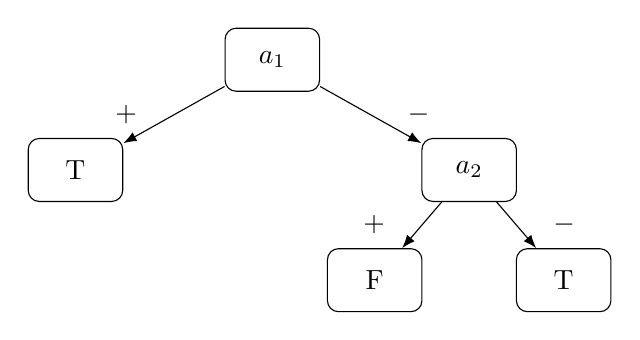
\begin{tikzpicture}[every node/.style={draw,rounded corners,minimum width=12mm,minimum height=8mm},
level distance=14mm,level 1/.style={sibling distance=50mm},level 2/.style={sibling distance=24mm},
edge from parent/.style={draw,-{Latex}}]
\node {$a_1$}
 child {node {T} edge from parent node[draw=none,left] {$+$}}
 child {node {$a_2$}
  child {node {F} edge from parent node[draw=none,left] {$+$}}
  child {node {T} edge from parent node[draw=none,right] {$-$}}
  edge from parent node[draw=none,right] {$-$}};
\end{tikzpicture}
\end{center}
\parttitle{(d) New instance}
For $a_1=+$ and $a_2=-$, the first split goes directly to T. The prediction is $\boxed{\mathrm{T}}$.

\parttitle{(e) Gini gain [CIS 5190]}
The parent Gini index is
\[
G(D)=1-\left(\frac34\right)^2-\left(\frac14\right)^2=0.375.
\]
For $a_1$, the child Gini indices are $0$ and $1-(1/2)^2-(1/2)^2=0.5$.
\[
G_{\text{children},a_1}=\frac24(0)+\frac24(0.5)=0.25,
\qquad \Delta G(a_1)=0.375-0.25=\boxed{0.125}.
\]
For $a_2$, the child Gini indices are $1-(2/3)^2-(1/3)^2=4/9$ and $0$.
\[
G_{\text{children},a_2}=\frac34\cdot\frac49+\frac14(0)=\frac13,
\qquad \Delta G(a_2)=\frac38-\frac13=\frac1{24}=\boxed{0.041667}.
\]
\end{document}
